\section{Introduction}
\label{sec:introduction}

% state the learning objective 
The objective of this laboratory assignment is to build an audio amplifier, increasing its gain and bandwidth and minimizing both cost and the value of the lower cutoff frequency. This audio amplifier is composed by gain and output stage.

As seen in Figure \ref{fig:rc}, this circuit has a supply voltage source with $Vcc=12 V$, and can be divided into four parts: \textbf{Input Voltage}, which is an sinusoidal (AC) signal $V_s$, it has a maximum amplitude of $10 mV$ and it's in series with a resistor $R_s=100 \Omega$; \textbf{Gain Stage},composed by a degenerated common emitter amplifier composed by a bias circuit with a bypass capacitor, and an NPN transistor; \textbf{Outuput Stage}, wchich is a common collector amplifier with a PNP transistor; \textbf{Output Voltage - Speaker}, which is the load of the circuit with $8 \Omega$.


\begin{figure}[h] \centering
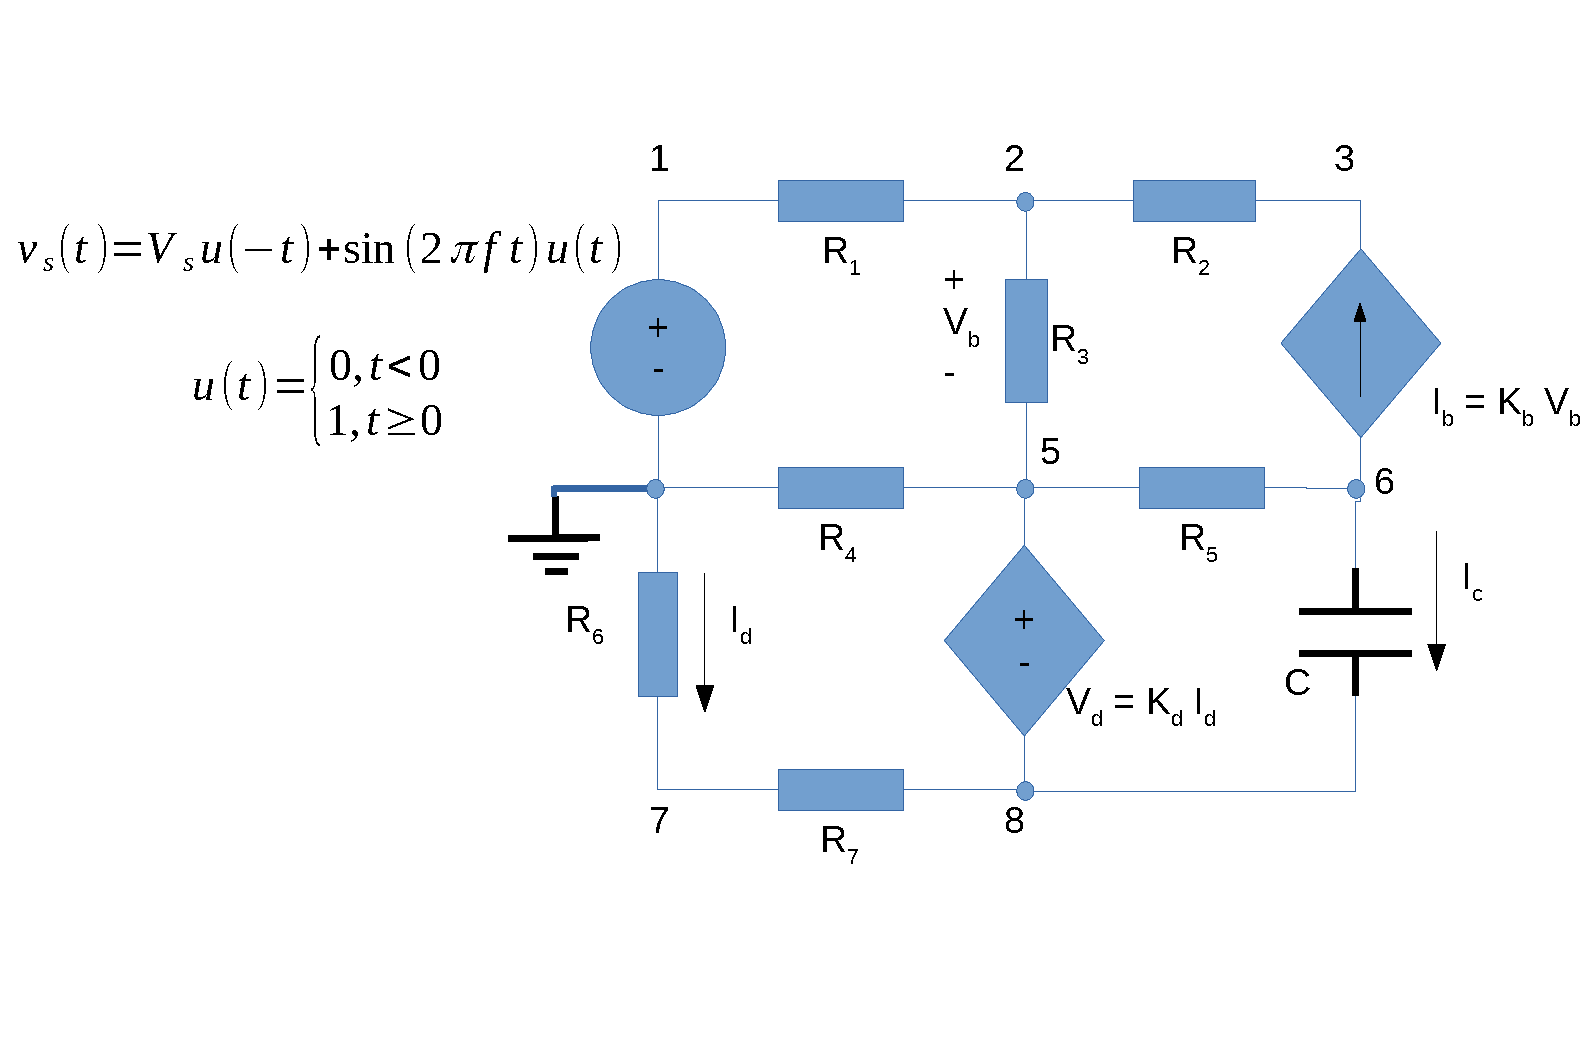
\includegraphics[width=0.99\linewidth]{rc.pdf}
\vspace{-5mm}
\caption{The Audio Amplifier}
\label{fig:rc}
\end{figure}



In Section \ref{sec:analysis}, a theoretical analysis of the circuit is presented. In Section\ref{sec:simulation}, the circuit is analysed by simulation, and the results are compared to the theoretical results obtained in Section\ref{sec:analysis}. The conclusions of this study are outlined in Section~\ref{sec:conclusion}.





